\documentclass[border=5pt]{standalone}
\usepackage{tikz}

\tikzset{
    every node/.style={
        text=black
    },
    every path/.style={
        color=black,
        thick
    }
}

\tikzstyle{pin}=[font=\ttfamily]

\begin{document}
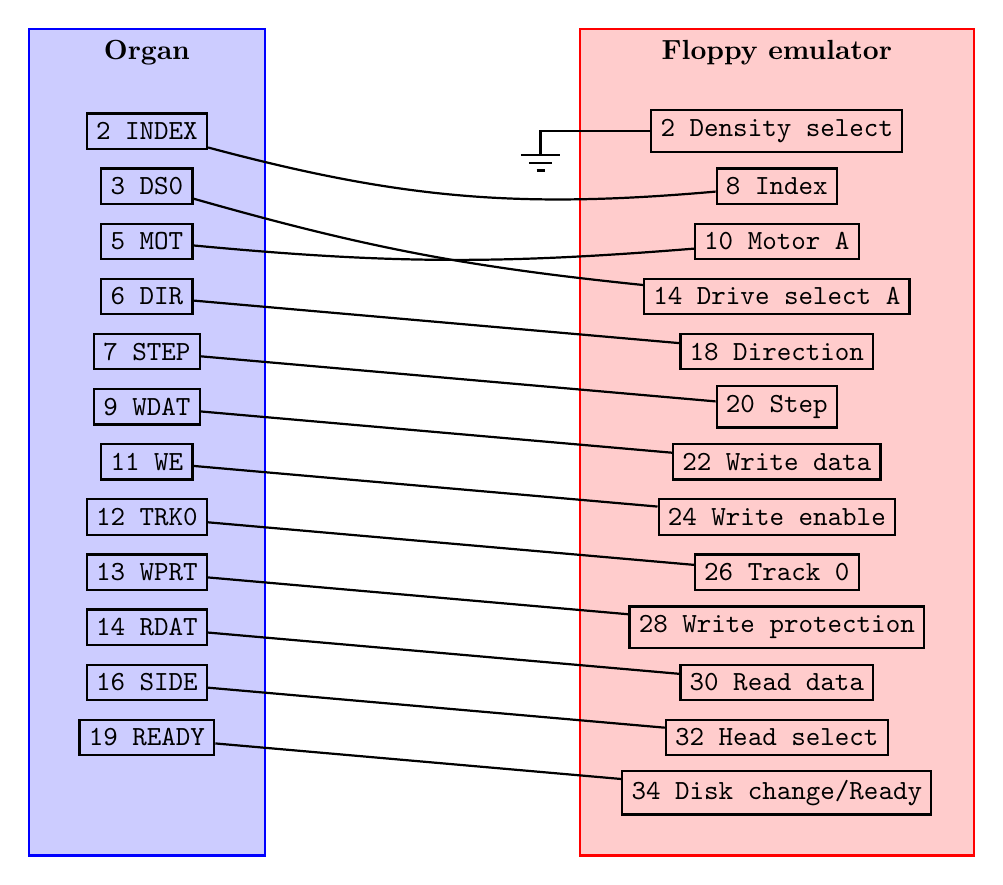
\begin{tikzpicture}
\draw[blue, fill=blue!20, thick] (0.5,0) rectangle (3.5,-10.5);
\draw[red, fill=red!20, thick] (7.5,0) rectangle (12.5,-10.5);

\node[anchor=center] at (2,-0.3) {\textbf{Organ}};
\node[anchor=center] at (10,-0.3) {\textbf{Floppy emulator}};

\node[pin,draw] (O2) at (2, -1.3) {2 INDEX};
\node[pin,draw] (O3) at (2, -2.0) {3 DS0};
\node[pin,draw] (O5) at (2, -2.7) {5 MOT};
\node[pin,draw] (O6) at (2, -3.4) {6 DIR};
\node[pin,draw] (O7) at (2, -4.1) {7 STEP};
\node[pin,draw] (O9) at (2, -4.8) {9 WDAT};
\node[pin,draw] (O11) at (2, -5.5) {11 WE};
\node[pin,draw] (O12) at (2, -6.2) {12 TRK0};
\node[pin,draw] (O13) at (2, -6.9) {13 WPRT};
\node[pin,draw] (O14) at (2, -7.6) {14 RDAT};
\node[pin,draw] (O16) at (2, -8.3) {16 SIDE};
\node[pin,draw] (O19) at (2, -9.0) {19 READY};

\node[pin,draw] (F2) at (10, -1.3) {2 Density select};
\node[pin,draw] (F8) at (10, -2.0) {8 Index};
\node[pin,draw] (F10) at (10, -2.7) {10 Motor A};
\node[pin,draw] (F14) at (10, -3.4) {14 Drive select A};
\node[pin,draw] (F18) at (10, -4.1) {18 Direction};
\node[pin,draw] (F20) at (10, -4.8) {20 Step};
\node[pin,draw] (F22) at (10, -5.5) {22 Write data};
\node[pin,draw] (F24) at (10, -6.2) {24 Write enable};
\node[pin,draw] (F26) at (10, -6.9) {26 Track 0};
\node[pin,draw] (F28) at (10, -7.6) {28 Write protection};
\node[pin,draw] (F30) at (10, -8.3) {30 Read data};
\node[pin,draw] (F32) at (10, -9.0) {32 Head select};
\node[pin,draw] (F34) at (10, -9.7) {34 Disk change/Ready};

\path [-] (O2) edge [bend right=10] (F8);
\path [-] (O3) edge [bend right=5] (F14);
\path [-] (O5) edge [bend right=5] (F10);
\path [-] (O6) edge (F18);
\path [-] (O7) edge (F20);
\path [-] (O9) edge (F22);
\path [-] (O11) edge (F24);
\path [-] (O12) edge (F26);
\path [-] (O13) edge (F28);
\path [-] (O14) edge (F30);
\path [-] (O16) edge (F32);
\path [-] (O19) edge (F34);

\draw (F2) -- (7, -1.3) -- (7, -1.6);
\path [-] (6.75, -1.6) edge (7.25, -1.6);
\path [-] (6.85, -1.7) edge (7.15, -1.7);
\path [-] (6.95, -1.8) edge (7.05, -1.8);

\end{tikzpicture}

\end{document}
